Κάποιες βασικές συναρτήσεις είναι:

\vspace{1em}

\textbf{Η πολυωνυμική συνάρτηση $f(x) = {\alpha}x + \beta$}
\begin{center}
\begin{tikzpicture}[scale=0.80, >=stealth]

  %%%%%%%%%%%%%%%%%%%%%%%%%%%%%%%%%%%%%%%%%%%%%%%%%
  \begin{scope}
    % Axes
    \draw[->, thick] (-2, 0) -- (2, 0) node[right] {$x$};
    \draw[->, thick] (0, -2) -- (0, 2) node[above] {$y$};

    % Plot function y = -sin(x) + 1.5
    \draw[domain=-2:1.5, smooth, variable=\x, blue, thick]
        plot ({\x},{0.7*\x + 0.5});

    % Vertical dotted arrows to x-axis

    % Origin and labels
    \node[below left] at (0,0) {$O$};

    \node at (-2.2,2) {$\alpha > 0$};
  \end{scope}

  %%%%%%%%%%%%%%%%%%%%%%%%%%%%%%%%%%%%%%%%%%%%%%%%%
  \begin{scope}[xshift=7.2cm]
    % Axes
    \draw[->, thick] (-2, 0) -- (2, 0) node[right] {$x$};
    \draw[->, thick] (0, -2) -- (0, 2) node[above] {$y$};

    % Plot function
    \draw[domain=-1:1.7, smooth, variable=\x, blue, thick]
        plot ({\x},{-1.3*\x + 0.5});


    % Origin and labels
    \node[below left] at (0,0) {$O$};

    \node at (-2.2,2) {$\alpha < 0$};
  \end{scope}

  %%%%%%%%%%%%%%%%%%%%%%%%%%%%%%%%%%%%%%%%%%%%%%%%%
  \begin{scope}[xshift=14.3cm]
    % Axes
    \draw[->, thick] (-2, 0) -- (2, 0) node[right] {$x$};
    \draw[->, thick] (0, -2) -- (0, 2) node[above] {$y$};

    % Plot function
    \draw[domain=-2:2, smooth, variable=\x, blue, thick]
        plot ({\x},{0.5});


    \node[below left] at (0,0) {$O$};

    \node at (-2.2,2) {$\alpha = 0$};
  \end{scope}

\end{tikzpicture}
\end{center}


\textbf{Η πολυωνυμική συνάρτηση $f(x) = {\alpha}x^2, \alpha \ne 0$}
\begin{center}
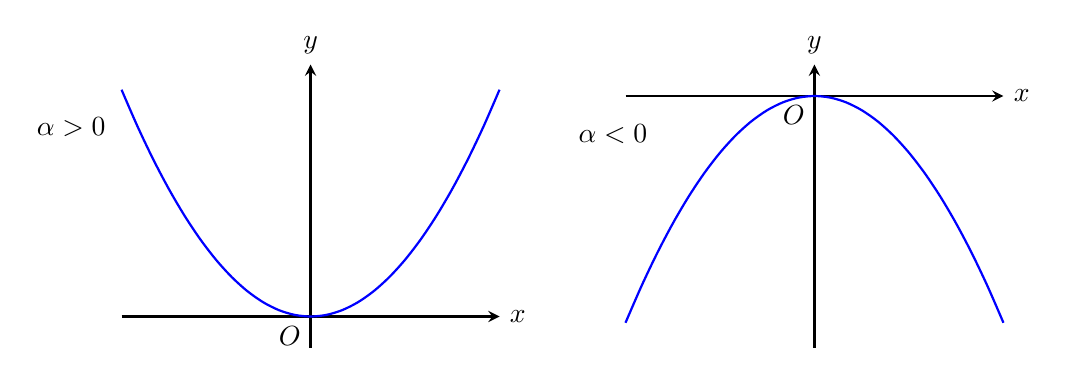
\begin{tikzpicture}[scale=0.8,>=stealth]

%%%%%%%%%%%%%%%%%%%%%%%%%%%%%%%%%%%%%%%%%%
  % Local scope
  \begin{scope}
    % Axes
    \draw[->, thick] (-3,0) -- (3,0) node[right] {$x$};
    \draw[->, thick] (0,-0.5) -- (0,4) node[above] {$y$};

    % Origin label
    \node[below left] at (0,0) {$O$};


    % Plot y = e^{x/5}
    \draw[domain=-3:3, smooth, variable=\x, blue, thick]
      plot ({\x},{0.4*(\x)^2});
    \node at (-3.8,3) {$\alpha > 0$};
  \end{scope}

%%%%%%%%%%%%%%%%%%%%%%%%%%%%%%%%%%%%%%%%%%

  \begin{scope}[xshift=8cm] % shift to the right
    % Axes
    \draw[->, thick] (-3,3.5) -- (3,3.5) node[right] {$x$};
    \draw[->, thick] (0,-0.5) -- (0,4) node[above] {$y$};

    % Origin
    \node[below left] at (0,3.5) {$O$};

    % Plot y = e^{x/5}
    \draw[domain=-3:3, smooth, variable=\x, blue, thick]
      plot ({\x},{-0.4*(\x)^2 + 3.5});
    \node at (-3.2,2.9) {$\alpha < 0$};
  \end{scope}

\end{tikzpicture}
\end{center}


\textbf{Η πολυωνυμική συνάρτηση $f(x) = {\alpha}x^3, \alpha \ne 0$}
\begin{center}
\begin{tikzpicture}[scale=0.8,>=stealth]

%%%%%%%%%%%%%%%%%%%%%%%%%%%%%%%%%%%%%%%%%%
  % Local scope
  \begin{scope}
    % Axes
    \draw[->, thick] (-3,0) -- (3,0) node[right] {$x$};
    \draw[->, thick] (0,-3) -- (0,3) node[above] {$y$};

    % Origin label
    \node[below left] at (0,0) {$O$};


    % Plot y = e^{x/5}
    \draw[domain=-2.8:2.8, smooth, variable=\x, blue, thick]
      plot ({\x},{0.15*(\x)^3});
    \node at (-3,3) {$\alpha > 0$};
  \end{scope}

%%%%%%%%%%%%%%%%%%%%%%%%%%%%%%%%%%%%%%%%%%

  \begin{scope}[xshift=9.1cm] % shift to the right
    % Axes
    \draw[->, thick] (-3,0) -- (3,0) node[right] {$x$};
    \draw[->, thick] (0,-3) -- (0,3) node[above] {$y$};

    % Origin
    \node[below left] at (0,0) {$O$};

    % Plot y = e^{x/5}
    \draw[domain=-2.8:2.8, smooth, variable=\x, blue, thick]
      plot ({\x},{-0.15*(\x)^3});

    \node at (-3.5,3) {$\alpha < 0$};

  \end{scope}

\end{tikzpicture}
\end{center}


\textbf{Η ρητή συνάρτηση $f(x) = \frac{\alpha}{x}, \alpha \ne 0$ και $D_{f} = \mathbb{R}^*$}
\begin{center}
\begin{tikzpicture}[scale=0.8,>=stealth]

%%%%%%%%%%%%%%%%%%%%%%%%%%%%%%%%%%%%%%%%%%
  % Local scope
  \begin{scope}
    % Axes
    \draw[->, thick] (-3,0) -- (3,0) node[right] {$x$};
    \draw[->, thick] (0,-3) -- (0,3) node[above] {$y$};

    % Origin label
    \node[below left] at (0,0) {$O$};


    % Plot y = e^{x/5}
    \draw[domain=0.17:2.8, smooth, variable=\x, blue, thick]
      plot ({\x},{0.5/(\x)});
    \draw[domain=-2.8:-0.17, smooth, variable=\x, blue, thick]
      plot ({\x},{0.5/(\x)});

    \node at (-2.6,3) {$\alpha > 0$};

  \end{scope}

%%%%%%%%%%%%%%%%%%%%%%%%%%%%%%%%%%%%%%%%%%

  \begin{scope}[xshift=9cm] % shift to the right
    % Axes
    \draw[->, thick] (-3,0) -- (3,0) node[right] {$x$};
    \draw[->, thick] (0,-3) -- (0,3) node[above] {$y$};

    % Origin
    \node[below left] at (0,0) {$O$};

    % Plot y = e^{x/5}
    \draw[domain=0.17:2.8, smooth, variable=\x, blue, thick]
      plot ({\x},{-0.5/(\x)});
    \draw[domain=-2.8:-0.17, smooth, variable=\x, blue, thick]
      plot ({\x},{-0.5/(\x)});

    \node at (-2.6,3) {$\alpha < 0$};
  \end{scope}

\end{tikzpicture}
\end{center}


\newpage

\textbf{Η συνάρτηση $f(x) = \sqrt{x}, \alpha \ne 0$ και $D_{f} = [0,+\infty)$}
\begin{center}
\begin{tikzpicture}[scale=0.8,>=stealth]

%%%%%%%%%%%%%%%%%%%%%%%%%%%%%%%%%%%%%%%%%%
  % Local scope
  \begin{scope}
    % Axes
    \draw[->, thick] (-0.5,0) -- (6,0) node[right] {$x$};
    \draw[->, thick] (0,-0.5) -- (0,5) node[above] {$y$};

    % Origin label
    \node[below left] at (0,0) {$O$};


    % Plot y = e^{x/5}
    \draw[domain=0:6, smooth, variable=\x, blue, thick]
      plot ({\x},{(\x)^(1/2)});

  \end{scope}
\end{tikzpicture}
\end{center}


\textbf{Η τριγωνομετρική συναρτήσεις: $f(x) = {\eta\mu}x, f(x) = {\sigma\upsilon\nu}x, f(x) = {\varepsilon\varphi}x$}
\begin{center}
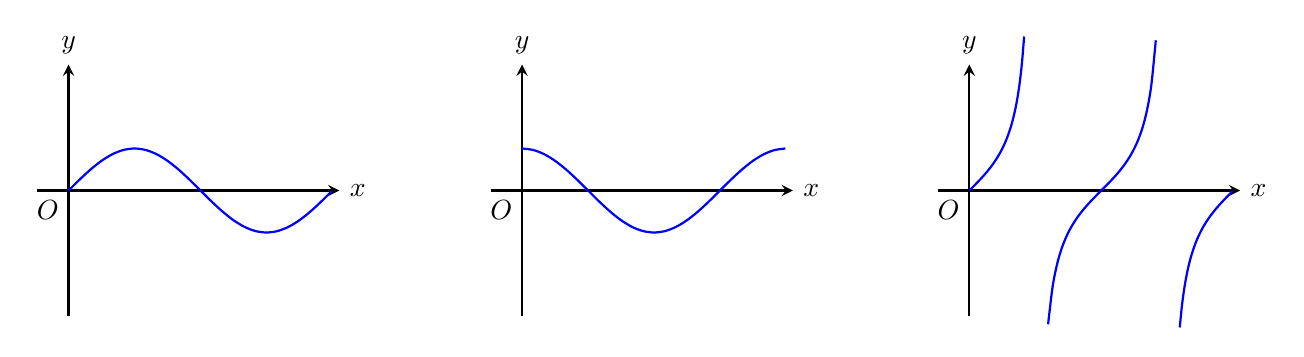
\begin{tikzpicture}[scale=0.80, >=stealth]

  %%%%%%%%%%%%%%%%%%%%%%%%%%%%%%%%%%%%%%%%%%%%%%%%%
  \begin{scope}
    % Axes
    \draw[->, thick] (-0.5, 0) -- (4.3, 0) node[right] {$x$};
    \draw[->, thick] (0, -2) -- (0, 2) node[above] {$y$};

    % Plot function y = -sin(x) + 1.5
    \draw[domain=0:4.18, smooth, variable=\x, blue, thick]
        plot ({\x},{sin(deg(\x*1.5))/1.5});

    % Vertical dotted arrows to x-axis

    % Origin and labels
    \node[below left] at (0,0) {$O$};
  \end{scope}

  %%%%%%%%%%%%%%%%%%%%%%%%%%%%%%%%%%%%%%%%%%%%%%%%%
  \begin{scope}[xshift=7.2cm]
    % Axes
    \draw[->, thick] (-0.5, 0) -- (4.3, 0) node[right] {$x$};
    \draw[->, thick] (0, -2) -- (0, 2) node[above] {$y$};

    % Plot function
    \draw[domain=0:4.18, smooth, variable=\x, blue, thick]
        plot ({\x},{cos(deg(\x*1.5))/1.5});

    % Origin and labels
    \node[below left] at (0,0) {$O$};
  \end{scope}

  %%%%%%%%%%%%%%%%%%%%%%%%%%%%%%%%%%%%%%%%%%%%%%%%%
  \begin{scope}[xshift=14.3cm]
    % Axes
    \draw[->, thick] (-0.5, 0) -- (4.3, 0) node[right] {$x$};
    \draw[->, thick] (0, -2) -- (0, 2) node[above] {$y$};

    % Plot function
    \draw[domain=0:0.87, smooth, variable=\x, blue, thick]
        plot ({\x},{tan(deg(\x*1.5))/1.5});

    % Plot function
    \draw[domain=1.25:2.96, smooth, variable=\x, blue, thick]
        plot ({\x},{tan(deg(\x*1.5))/1.5});

    % Plot function
    \draw[domain=3.34:4.18, smooth, variable=\x, blue, thick]
        plot ({\x},{tan(deg(\x*1.5))/1.5});


    \node[below left] at (0,0) {$O$};
  \end{scope}

\end{tikzpicture}
\end{center}


% Βασικές ιδιότητες γραφικών παραστάσεων
% !TeX root = ../../mathimatikaglykeiou.tex

Τέλος, γνωρίζοντας την γραφική παράσταση μιας συνάρτησης (δηλαδή την $C_{f}$), μπορούμαι εύκολα να υπολογίσουμε την γραφική παράσταση μιας συνάρτησης σε αυτές τις περιπτώσεις, έστω υπάρχει $f(x)$:
\begin{enumerate}
 \item $-f(x)$
 \item $\vert f(x) \vert$
 \item $f(-x)$ (εφόσον $-x \in D_{f}$)
 \item $f(\vert x\vert)$ (εφόσον $\vert x\vert \in D_{f}$)
\end{enumerate}

Άρα έστω η παρακάτω γραφική παράσταση συνάρτησης, $C_{f}$:

\begin{center}
\begin{tikzpicture}[scale=0.8,>=stealth]

%%%%%%%%%%%%%%%%%%%%%%%%%%%%%%%%%%%%%%%%%%
  % Local scope
  \begin{scope}
    % Axes
    \draw[->, thick] (-2,0) -- (5,0) node[right] {$x$};
    \draw[->, thick] (0,-0.5) -- (0,5) node[above] {$y$};

    % Origin label
    \node[below right] at (0,0) {$O$};


    % Plot y = e^{x/5}
    \draw[domain=-0.74:3.8, smooth, variable=\x, blue, thick]
      plot ({\x},{-( ((-\x +1)/1.9)^7 + ((-\x +1)/1.9)^6 + ((-\x +1)/1.9)^2 + 2) + 2.7});

  \end{scope}
\end{tikzpicture}
\end{center}

Μπορούμαι να σχεδιάσουμε τις παρακάτω συναρτήσεις:

\begin{center}
\begin{tikzpicture}[scale=0.8,>=stealth]

%%%%%%%%%%%%%%%%%%%%%%%%%%%%%%%%%%%%%%%%%%
  % Local scope
  \begin{scope}
    % Axes
    \draw[->, thick] (-1.5,0) -- (4,0) node[right] {$x$};
    \draw[->, thick] (0,-3.6) -- (0,3.6) node[above] {$y$};

    % Origin label
    \node[below right] at (0,0) {$O$};


    \draw[domain=-1:3.7, dotted, variable=\x, blue, thick]
      plot ({\x},{-( ((-\x +1)/1.9)^7 + ((-\x +1)/1.9)^6 + ((-\x +1)/1.9)^2 + 2) + 2.7});
    \draw[domain=-1:3.7, smooth, variable=\x, blue, thick]
      plot ({\x},{( ((-\x +1)/1.9)^7 + ((-\x +1)/1.9)^6 + ((-\x +1)/1.9)^2 + 2) - 2.7});
    \node at (-1.9,-3.6) {(1)};

  \end{scope}

%%%%%%%%%%%%%%%%%%%%%%%%%%%%%%%%%%%%%%%%%%

  \begin{scope}[xshift=9cm] % shift to the right
    % Axes
    \draw[->, thick] (-1.5,0) -- (4,0) node[right] {$x$};
    \draw[->, thick] (0,-3.6) -- (0,3.6) node[above] {$y$};

    % Origin
    \node[below left] at (0,0) {$O$};


    \draw[domain=-1:3.7, dotted, variable=\x, blue, thick]
      plot ({\x},{-( ((-\x +1)/1.9)^7 + ((-\x +1)/1.9)^6 + ((-\x +1)/1.9)^2 + 2) + 2.7});
    \draw[domain=-1:3.7, samples=200, smooth, variable=\x, blue, thick]
      plot ({\x},{abs(-( ((-\x +1)/1.9)^7 + ((-\x +1)/1.9)^6 + ((-\x +1)/1.9)^2 + 2) + 2.7)});
    \node at (-1.9,-3.6) {(2)};
  \end{scope}

\end{tikzpicture}
\end{center}

\begin{center}
\begin{tikzpicture}[scale=0.8,>=stealth]

  \begin{scope} % shift to the right
    % Axes
    \draw[->, thick] (-4,0) -- (4,0) node[right] {$x$};
    \draw[->, thick] (0,-3.6) -- (0,3.6) node[above] {$y$};

    % Origin
    \node[below left] at (0,0) {$O$};

    \draw[domain=-1:3.7, dotted, variable=\x, blue, thick]
      plot ({\x},{-( ((-\x +1)/1.9)^7 + ((-\x +1)/1.9)^6 + ((-\x +1)/1.9)^2 + 2) + 2.7});
    \draw[domain=-1:3.7, smooth, variable=\x, blue, thick]
      plot ({-\x},{-( ((-\x +1)/1.9)^7 + ((-\x +1)/1.9)^6 + ((-\x +1)/1.9)^2 + 2) + 2.7});

    \node at (-3.5,-3.6) {(3)};
  \end{scope}

  \begin{scope}[xshift=9.1cm] % shift to the right
    % Axes
    \draw[->, thick] (-4,0) -- (4,0) node[right] {$x$};
    \draw[->, thick] (0,-3.6) -- (0,3.6) node[above] {$y$};

    % Origin
    \node[below right] at (0,0) {$O$};

    \draw[domain=-1:3.7, dotted, variable=\x, blue, thick]
      plot ({\x},{-( ((-\x +1)/1.9)^7 + ((-\x +1)/1.9)^6 + ((-\x +1)/1.9)^2 + 2) + 2.7});
    \draw[domain=-3.7:3.7, samples=200, smooth, variable=\x, blue, thick]
      plot ({\x},{-( ((-abs(\x) +1)/1.9)^7 + ((-abs(\x) +1)/1.9)^6 + ((-abs(\x) +1)/1.9)^2 + 2) + 2.7});

    \node at (-3.5,-3.6) {(4)};
  \end{scope}
\end{tikzpicture}
\end{center}


\textbf{ΠΡΟΣΟΧΗ!!!} Αν υποθέσουμε ότι το πεδίο ορισμού της συνάρτησης είναι αυτό που δόθηκε στο $C_f$, τότε: Οι δύο τελευταίες γραφικές παραστάσεις ((3),(4)) \textbf{\textit{δεν}} αναπαριστώνται στο πεδίο ορισμού που έχει δοθεί για το $C_f$.



{\large \textbf{- Μετατόπιση Συνάρτησης}}
\vspace{1em}

Επιπλέον, η οριζόντια και η κατακόρυφη μετατόπιση γίνεται ως εξής:

Έστω $f: A \to \mathbb{R}$, και η γραφική παράσταση της $C_{f}$. Επίσης έστω $\alpha \in \mathbb{R}$.

\begin{center}
\begin{tikzpicture}[scale=1, >=stealth]

  %%%%%%%%%%%%%%%%%%%%%%%%%%%%%%%%%%%%%%%%%%%%%%%%%
  \begin{scope}
    % Axes
    \draw[->, thick] (-0.5, 0) -- (5.5, 0) node[right] {$x$};
    \draw[->, thick] (0, -0.5) -- (0, 3) node[above] {$y$};

    % Plot function y = -sin(x) + 1.5
    \draw[domain=1:5, smooth, variable=\x, red, thick]
        plot ({\x},{-sin(deg(\x)) + 2});

    \draw[domain=1:5, smooth, variable=\x, blue, thick]
        plot ({\x},{-sin(deg(\x)) + 0.5});


    \draw[decorate, decoration={brace, mirror, amplitude=6pt}, thick]
        (5.2, 1.45) -- (5.2, 2.95);

    \node[right] at (5.4,2.2) {$\alpha$};

    % Origin and labels
    \node[below left] at (0,0) {$O$};
    \node at (3.8,0.5) {$C_{f}$};

    \node at (3,-1.3) {$f(x) + \alpha$, όταν $\alpha > 0$};

    \tikzset{dot/.style={circle, fill=red, inner sep=1.5pt}}
    \node[dot] (a1) at (1,1.15) {};
    \node[dot] (a2) at (5,2.95) {};

    \tikzset{dot/.style={circle, fill=blue, inner sep=1.5pt}}
    \node[dot] (a3) at (1,-0.35) {};
    \node[dot] (a4) at (5,1.45) {};
    % Vertical dotted arrows to x-axis
    \foreach \x in {1,1.5,...,5}
        \draw[dotted, thick, ->] (\x, {-sin(deg(\x)) + 0.5}) -- (\x, {-sin(deg(\x)) + 2});
  \end{scope}

  %%%%%%%%%%%%%%%%%%%%%%%%%%%%%%%%%%%%%%%%%%%%%%%%%
  \begin{scope}[xshift=7.2cm]
    % Axes
    \draw[->, thick] (-0.5, 0) -- (5.5, 0) node[right] {$x$};
    \draw[->, thick] (0, -0.5) -- (0, 3) node[above] {$y$};

    % Plot function y = -sin(x) + 1.5
    \draw[domain=1:5, smooth, variable=\x, blue, thick]
        plot ({\x},{-sin(deg(\x)) + 2.4});

    \draw[domain=1:5, smooth, variable=\x, red, thick]
        plot ({\x},{-sin(deg(\x)) + 1.3});

    \draw[decorate, decoration={brace, mirror, amplitude=6pt}, thick]
        (5.2, 2.25) -- (5.2, 3.35);

    \node[right] at (5.4,2.8) {$\alpha$};
    % Vertical dotted arrows to x-axis


    % Origin and labels
    \node[below left] at (0,0) {$O$};
    \node at (3,3) {$C_{f}$};

    \node at (3,-1.3) {$f(x) + \alpha$, όταν $\alpha < 0$};

    \tikzset{dot/.style={circle, fill=blue, inner sep=1.5pt}}
    \node[dot] (a1) at (1,1.55) {};
    \node[dot] (a2) at (5,3.35) {};

    \tikzset{dot/.style={circle, fill=red, inner sep=1.5pt}}
    \node[dot] (a3) at (1,0.45) {};
    \node[dot] (a4) at (5,2.25) {};

    \foreach \x in {1,1.5,...,5}
        \draw[dotted, thick, ->] (\x, {-sin(deg(\x)) + 2.4}) -- (\x, {-sin(deg(\x)) + 1.3});
  \end{scope}

\end{tikzpicture}

\end{center}

\begin{center}
\begin{tikzpicture}[scale=1, >=stealth]

  %%%%%%%%%%%%%%%%%%%%%%%%%%%%%%%%%%%%%%%%%%%%%%%%%
  \begin{scope}
    % Axes
    \draw[->, thick] (-0.5, 0.6) -- (5.5, 0.6) node[right] {$x$};
    \draw[->, thick] (2.5, -0.5) -- (2.5, 3) node[above] {$y$};

    % Plot function y = -sin(x) + 1.5
    \draw[domain=2.2:5.3, smooth, variable=\x, red, thick]
        plot ({\x},{ln(\x - 2) + 1.6});
    \draw[domain=0.6:3.7, smooth, variable=\x, blue, thick]
        plot ({\x},{ln(\x - 0.4) + 1.6});

    \draw[decorate, decoration={brace, amplitude=6pt}, thick]
        (3.7, 2.9) -- (5.3, 2.9);

    \node[above] at (4.5,3) {$\alpha$};

    % Origin and labels
    \node[below left] at (0,0) {$O$};
    \node at (1.3,2.2) {$C_{f}$};

    \node at (3,-1.3) {$f(x + \alpha)$, όταν $\alpha > 0$};

    \tikzset{dot/.style={circle, fill=red, inner sep=1.5pt}}
    \node[dot] (a1) at (2.2,0) {};
    \node[dot] (a2) at (5.3,2.79) {};

    \tikzset{dot/.style={circle, fill=blue, inner sep=1.5pt}}
    \node[dot] (a3) at (0.6,0) {};
    \node[dot] (a4) at (3.7,2.79) {};

    % Vertical dotted arrows to x-axis
    \foreach \y in {0,0.398,...,2.79}
        \draw[dotted, thick, ->] ({e^(\y - 1.6) + 0.4}, \y) -- ({e^(\y - 1.6) + 2}, \y);
  \end{scope}

  %%%%%%%%%%%%%%%%%%%%%%%%%%%%%%%%%%%%%%%%%%%%%%%%%
  \begin{scope}[xshift=7.2cm]
    % Axes
    \draw[->, thick] (-0.5, 0.6) -- (5.5, 0.6) node[right] {$x$};
    \draw[->, thick] (2.5, -0.5) -- (2.5, 3) node[above] {$y$};

    % Plot function y = -sin(x) + 1.5
    \draw[domain=2.2:5.3, smooth, variable=\x, blue, thick]
        plot ({\x},{ln(\x - 2) + 1.6});
    \draw[domain=0.6:3.7, smooth, variable=\x, red, thick]
        plot ({\x},{ln(\x - 0.4) + 1.6});
    \draw[decorate, decoration={brace, amplitude=6pt}, thick]
        (3.7, 2.9) -- (5.3, 2.9);

    \node[above] at (4.5,3) {$\alpha$};

    % Origin and labels
    \node[below left] at (0,0) {$O$};
    \node at (4,1.7) {$C_{f}$};

    \node at (3,-1.3) {$f(x + \alpha)$, όταν $\alpha < 0$};

    \tikzset{dot/.style={circle, fill=blue, inner sep=1.5pt}}
    \node[dot] (a1) at (2.2,0) {};
    \node[dot] (a2) at (5.3,2.79) {};

    \tikzset{dot/.style={circle, fill=red, inner sep=1.5pt}}
    \node[dot] (a3) at (0.6,0) {};
    \node[dot] (a4) at (3.7,2.79) {};

    % Vertical dotted arrows to x-axis
    \foreach \y in {0,0.398,...,2.79}
        \draw[dotted, thick, ->] ({e^(\y - 1.6) + 2}, \y) -- ({e^(\y - 1.6) + 0.4}, \y);
  \end{scope}

\end{tikzpicture}

\end{center}

\textbf{ΠΡΟΣΟΧΗ!!!} Για να ισχύοουν τα δύο τελευταία παραδείγματα πρέπει $x + \alpha \in A$, όπου $A$ είναι το πεδίο ορισμού της συνάρτησης $f$.

